\documentclass{ximera}
\input{../preamble.tex}

\author{Robert Kenney \and Paul Zachlin \and Nicholas Shay}
\title{X-bar Charts} \license{CC BY-NC-SA 4.0}
\begin{document}

\begin{abstract}
We study basic ideas behind the use of control charts in industry.
\end{abstract}
\maketitle

\begin{onlineOnly}
\section*{X-bar Charts}
\end{onlineOnly}

In the last section we introduced two kinds of control charts, x-bar chart and R-chart.  In this section we will 




\subsection*{When is it time to investigate?}

\href{https://www.qimacros.com/control-chart/nelson-rules/}{Nelson rules} for detecting an out-of-control process:

Rule 1:  One point falls above UCL or below LCL.

\begin{center}
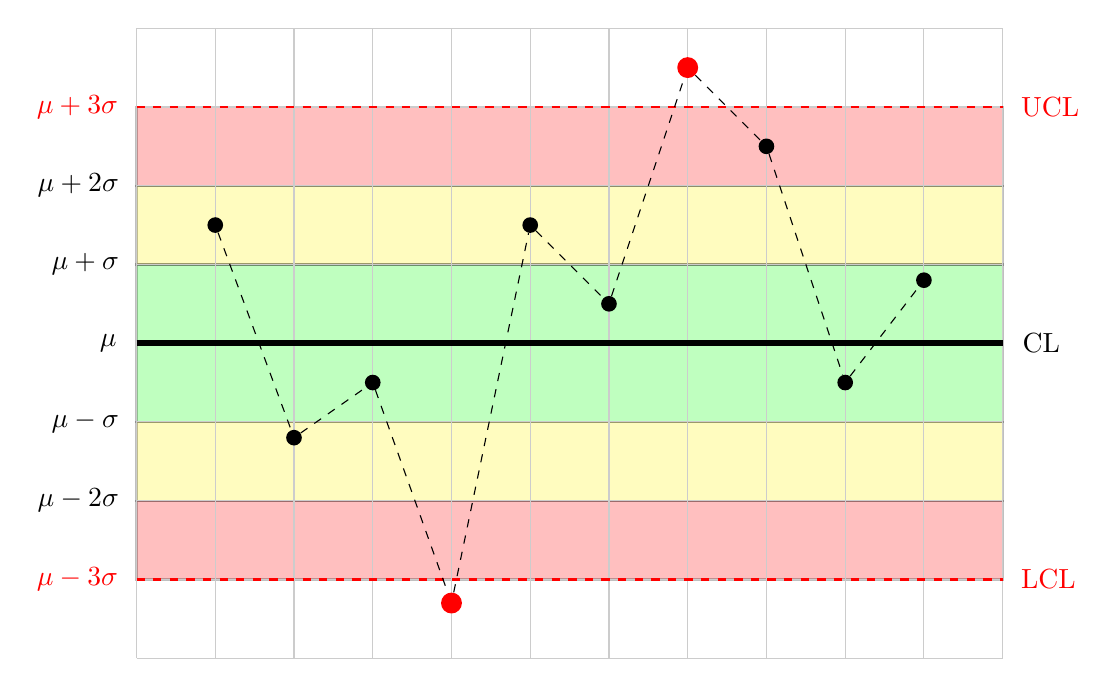
\begin{tikzpicture}[scale=1]
\draw[black, thick, fill=green,opacity=0.25] (0,-1) rectangle (11, 1);
\draw[black, thick, fill=yellow,opacity=0.25] (0,-2) rectangle (11, -1);
\draw[black, thick, fill=yellow,opacity=0.25] (0,1) rectangle (11, 2);
\draw[black, thick, fill=red,opacity=0.25] (0,-3) rectangle (11, -2);
\draw[black, thick, fill=red,opacity=0.25] (0,2) rectangle (11, 3);
\draw[thin,gray!40] (0,-4) grid (11,4);
\draw[line width=2pt](0,0)node[left=1mm]{$\mu$}--(11,0)node[right=1mm]{CL} ;
 \draw[line width=1pt,red, dashed](0,3)node[left=1mm]{$\mu+3\sigma$}--(11,3)node[right=1mm]{UCL};
\draw[line width=1pt,red, dashed](0,-3)node[left=1mm]{$\mu-3\sigma$}--(11,-3)node[right=1mm]{LCL};

\node[left=1mm] at (0,1){$\mu+\sigma$};
\node[left=1mm] at (0,-1){$\mu-\sigma$};
\node[left=1mm] at (0,2){$\mu+2\sigma$};
\node[left=1mm] at (0,-2){$\mu-2\sigma$};

 \node (A) at (1,1.5) [circle,fill=black,scale=0.6]{};
 \node (B) at (2,-1.2) [circle,fill=black,scale=0.6]{};
 \node (C) at (3,-0.5) [circle,fill=black,scale=0.6]{};
 \node (D) at (4,-3.3) [circle,fill=red,scale=0.8]{};
 \node (E) at (5,1.5) [circle,fill=black,scale=0.6]{};
 \node (F) at (6,0.5) [circle,fill=black,scale=0.6]{};
\node (G) at (7,3.5) [circle,fill=red,scale=0.8]{};
\node (H) at (8,2.5) [circle,fill=black,scale=0.6]{};
\node (I) at (9,-0.5) [circle,fill=black,scale=0.6]{};
\node (J) at (10,0.8) [circle,fill=black,scale=0.6]{};

\draw[-,dashed] (A)--(B); 
\draw[-,dashed] (B)--(C);
\draw[-,dashed] (C)--(D);
\draw[-,dashed] (D)--(E); 
\draw[-,dashed] (E)--(F);
\draw[-,dashed] (F)--(G); 
\draw[-,dashed] (G)--(H);
\draw[-,dashed] (H)--(I);
\draw[-,dashed] (I)--(J);

 \end{tikzpicture}
\end{center}

Rule 2:  Two out of three consecutive points are on the same side of the center line and above $\mu+2\sigma$ or below $\mu-2\sigma$.

\begin{center}
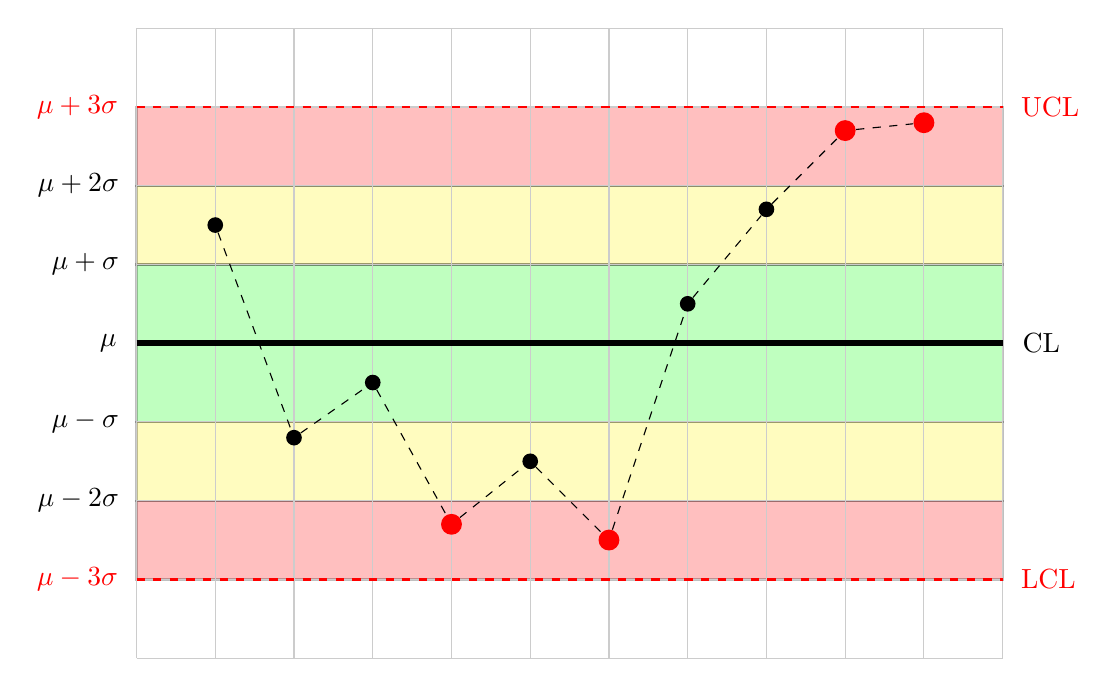
\begin{tikzpicture}[scale=1]
\draw[black, thick, fill=green,opacity=0.25] (0,-1) rectangle (11, 1);
\draw[black, thick, fill=yellow,opacity=0.25] (0,-2) rectangle (11, -1);
\draw[black, thick, fill=yellow,opacity=0.25] (0,1) rectangle (11, 2);
\draw[black, thick, fill=red,opacity=0.25] (0,-3) rectangle (11, -2);
\draw[black, thick, fill=red,opacity=0.25] (0,2) rectangle (11, 3);
\draw[thin,gray!40] (0,-4) grid (11,4);
\draw[line width=2pt](0,0)node[left=1mm]{$\mu$}--(11,0)node[right=1mm]{CL} ;
 \draw[line width=1pt,red, dashed](0,3)node[left=1mm]{$\mu+3\sigma$}--(11,3)node[right=1mm]{UCL};
\draw[line width=1pt,red, dashed](0,-3)node[left=1mm]{$\mu-3\sigma$}--(11,-3)node[right=1mm]{LCL};

\node[left=1mm] at (0,1){$\mu+\sigma$};
\node[left=1mm] at (0,-1){$\mu-\sigma$};
\node[left=1mm] at (0,2){$\mu+2\sigma$};
\node[left=1mm] at (0,-2){$\mu-2\sigma$};

 \node (A) at (1,1.5) [circle,fill=black,scale=0.6]{};
 \node (B) at (2,-1.2) [circle,fill=black,scale=0.6]{};
 \node (C) at (3,-0.5) [circle,fill=black,scale=0.6]{};
 \node (D) at (4,-2.3) [circle,fill=red,scale=0.8]{};
 \node (E) at (5,-1.5) [circle,fill=black,scale=0.6]{};
 \node (F) at (6,-2.5) [circle,fill=red,scale=0.8]{};
\node (G) at (7,0.5) [circle,fill=black,scale=0.6]{};
\node (H) at (8,1.7) [circle,fill=black,scale=0.6]{};
\node (I) at (9,2.7) [circle,fill=red,scale=0.8]{};
\node (J) at (10,2.8) [circle,fill=red,scale=0.8]{};

\draw[-,dashed] (A)--(B); 
\draw[-,dashed] (B)--(C);
\draw[-,dashed] (C)--(D);
\draw[-,dashed] (D)--(E); 
\draw[-,dashed] (E)--(F);
\draw[-,dashed] (F)--(G); 
\draw[-,dashed] (G)--(H);
\draw[-,dashed] (H)--(I);
\draw[-,dashed] (I)--(J);

 \end{tikzpicture}
\end{center}

Rule 3: Four out of five points are on the same side of the center line and above $\mu+\sigma$ or below $\mu-\sigma$.

\begin{center}
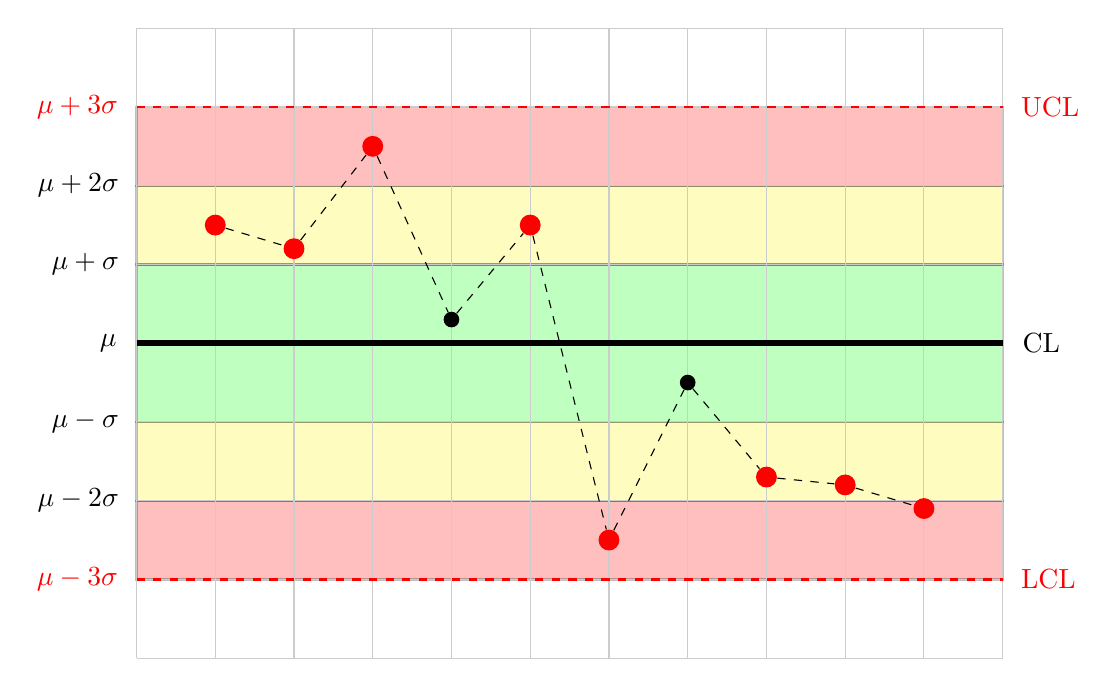
\begin{tikzpicture}[scale=1]
\draw[black, thick, fill=green,opacity=0.25] (0,-1) rectangle (11, 1);
\draw[black, thick, fill=yellow,opacity=0.25] (0,-2) rectangle (11, -1);
\draw[black, thick, fill=yellow,opacity=0.25] (0,1) rectangle (11, 2);
\draw[black, thick, fill=red,opacity=0.25] (0,-3) rectangle (11, -2);
\draw[black, thick, fill=red,opacity=0.25] (0,2) rectangle (11, 3);
\draw[thin,gray!40] (0,-4) grid (11,4);
\draw[line width=2pt](0,0)node[left=1mm]{$\mu$}--(11,0)node[right=1mm]{CL} ;
 \draw[line width=1pt,red, dashed](0,3)node[left=1mm]{$\mu+3\sigma$}--(11,3)node[right=1mm]{UCL};
\draw[line width=1pt,red, dashed](0,-3)node[left=1mm]{$\mu-3\sigma$}--(11,-3)node[right=1mm]{LCL};

\node[left=1mm] at (0,1){$\mu+\sigma$};
\node[left=1mm] at (0,-1){$\mu-\sigma$};
\node[left=1mm] at (0,2){$\mu+2\sigma$};
\node[left=1mm] at (0,-2){$\mu-2\sigma$};

 \node (A) at (1,1.5) [circle,fill=red,scale=0.8]{};
 \node (B) at (2,1.2) [circle,fill=red,scale=0.8]{};
 \node (C) at (3,2.5) [circle,fill=red,scale=0.8]{};
 \node (D) at (4,0.3) [circle,fill=black,scale=0.6]{};
 \node (E) at (5,1.5) [circle,fill=red,scale=0.8]{};
 \node (F) at (6,-2.5) [circle,fill=red,scale=0.8]{};
\node (G) at (7,-0.5) [circle,fill=black,scale=0.6]{};
\node (H) at (8,-1.7) [circle,fill=red,scale=0.8]{};
\node (I) at (9,-1.8) [circle,fill=red,scale=0.8]{};
\node (J) at (10,-2.1) [circle,fill=red,scale=0.8]{};

\draw[-,dashed] (A)--(B); 
\draw[-,dashed] (B)--(C);
\draw[-,dashed] (C)--(D);
\draw[-,dashed] (D)--(E); 
\draw[-,dashed] (E)--(F);
\draw[-,dashed] (F)--(G); 
\draw[-,dashed] (G)--(H);
\draw[-,dashed] (H)--(I);
\draw[-,dashed] (I)--(J);

 \end{tikzpicture}
\end{center}

Rule 4: Eight consecutive points are on the same side of the center line.

\begin{center}
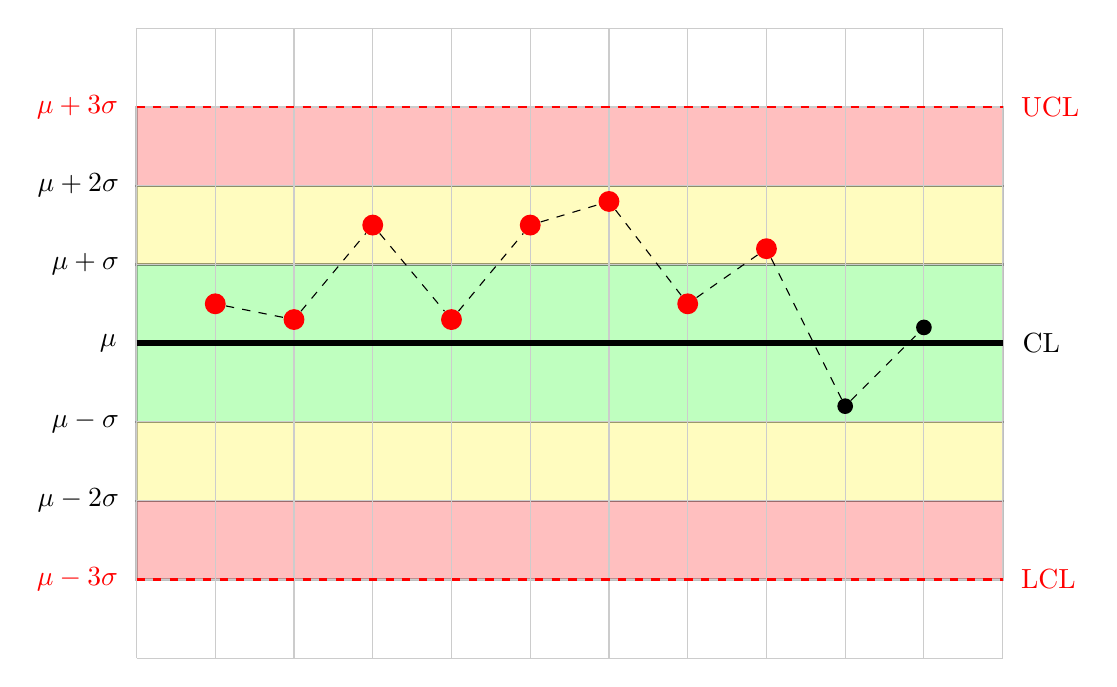
\begin{tikzpicture}[scale=1]
\draw[black, thick, fill=green,opacity=0.25] (0,-1) rectangle (11, 1);
\draw[black, thick, fill=yellow,opacity=0.25] (0,-2) rectangle (11, -1);
\draw[black, thick, fill=yellow,opacity=0.25] (0,1) rectangle (11, 2);
\draw[black, thick, fill=red,opacity=0.25] (0,-3) rectangle (11, -2);
\draw[black, thick, fill=red,opacity=0.25] (0,2) rectangle (11, 3);
\draw[thin,gray!40] (0,-4) grid (11,4);
\draw[line width=2pt](0,0)node[left=1mm]{$\mu$}--(11,0)node[right=1mm]{CL} ;
 \draw[line width=1pt,red, dashed](0,3)node[left=1mm]{$\mu+3\sigma$}--(11,3)node[right=1mm]{UCL};
\draw[line width=1pt,red, dashed](0,-3)node[left=1mm]{$\mu-3\sigma$}--(11,-3)node[right=1mm]{LCL};

\node[left=1mm] at (0,1){$\mu+\sigma$};
\node[left=1mm] at (0,-1){$\mu-\sigma$};
\node[left=1mm] at (0,2){$\mu+2\sigma$};
\node[left=1mm] at (0,-2){$\mu-2\sigma$};

 \node (A) at (1,0.5) [circle,fill=red,scale=0.8]{};
 \node (B) at (2,0.3) [circle,fill=red,scale=0.8]{};
 \node (C) at (3,1.5) [circle,fill=red,scale=0.8]{};
 \node (D) at (4,0.3) [circle,fill=red,scale=0.8]{};
 \node (E) at (5,1.5) [circle,fill=red,scale=0.8]{};
 \node (F) at (6,1.8) [circle,fill=red,scale=0.8]{};
\node (G) at (7,0.5) [circle,fill=red,scale=0.8]{};
\node (H) at (8,1.2) [circle,fill=red,scale=0.8]{};
\node (I) at (9,-0.8) [circle,fill=black,scale=0.6]{};
\node (J) at (10,0.2) [circle,fill=black,scale=0.6]{};

\draw[-,dashed] (A)--(B); 
\draw[-,dashed] (B)--(C);
\draw[-,dashed] (C)--(D);
\draw[-,dashed] (D)--(E); 
\draw[-,dashed] (E)--(F);
\draw[-,dashed] (F)--(G); 
\draw[-,dashed] (G)--(H);
\draw[-,dashed] (H)--(I);
\draw[-,dashed] (I)--(J);

 \end{tikzpicture}
\end{center}

Rule 5: Six consecutive points are ascending/decending. 

\begin{center}
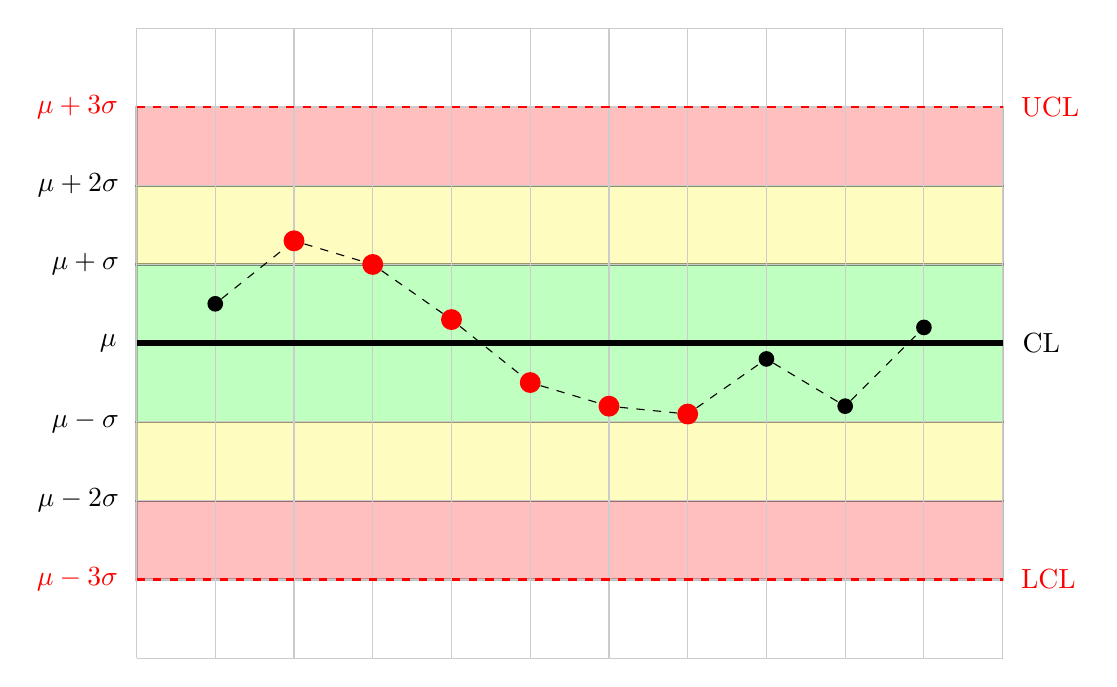
\begin{tikzpicture}[scale=1]
\draw[black, thick, fill=green,opacity=0.25] (0,-1) rectangle (11, 1);
\draw[black, thick, fill=yellow,opacity=0.25] (0,-2) rectangle (11, -1);
\draw[black, thick, fill=yellow,opacity=0.25] (0,1) rectangle (11, 2);
\draw[black, thick, fill=red,opacity=0.25] (0,-3) rectangle (11, -2);
\draw[black, thick, fill=red,opacity=0.25] (0,2) rectangle (11, 3);
\draw[thin,gray!40] (0,-4) grid (11,4);
\draw[line width=2pt](0,0)node[left=1mm]{$\mu$}--(11,0)node[right=1mm]{CL} ;
 \draw[line width=1pt,red, dashed](0,3)node[left=1mm]{$\mu+3\sigma$}--(11,3)node[right=1mm]{UCL};
\draw[line width=1pt,red, dashed](0,-3)node[left=1mm]{$\mu-3\sigma$}--(11,-3)node[right=1mm]{LCL};

\node[left=1mm] at (0,1){$\mu+\sigma$};
\node[left=1mm] at (0,-1){$\mu-\sigma$};
\node[left=1mm] at (0,2){$\mu+2\sigma$};
\node[left=1mm] at (0,-2){$\mu-2\sigma$};

 \node (A) at (1,0.5) [circle,fill=black,scale=0.6]{};
 \node (B) at (2,1.3) [circle,fill=red,scale=0.8]{};
 \node (C) at (3,1) [circle,fill=red,scale=0.8]{};
 \node (D) at (4,0.3) [circle,fill=red,scale=0.8]{};
 \node (E) at (5,-0.5) [circle,fill=red,scale=0.8]{};
 \node (F) at (6,-0.8) [circle,fill=red,scale=0.8]{};
\node (G) at (7,-0.9) [circle,fill=red,scale=0.8]{};
\node (H) at (8,-0.2) [circle,fill=black,scale=0.6]{};
\node (I) at (9,-0.8) [circle,fill=black,scale=0.6]{};
\node (J) at (10,0.2) [circle,fill=black,scale=0.6]{};

\draw[-,dashed] (A)--(B); 
\draw[-,dashed] (B)--(C);
\draw[-,dashed] (C)--(D);
\draw[-,dashed] (D)--(E); 
\draw[-,dashed] (E)--(F);
\draw[-,dashed] (F)--(G); 
\draw[-,dashed] (G)--(H);
\draw[-,dashed] (H)--(I);
\draw[-,dashed] (I)--(J);

 \end{tikzpicture}
\end{center}

Rule 6: Fifteen consecutive points are between $\mu-\sigma$ and $\mu+\sigma$.  This is known as ``hugging the center line".

Rule 7: Fourteen consecutive points form an alternating up/down pattern.

Rule 8:  Eight consecutive points are above $\mu+\sigma$ or below $\mu-\sigma$.

\begin{center}
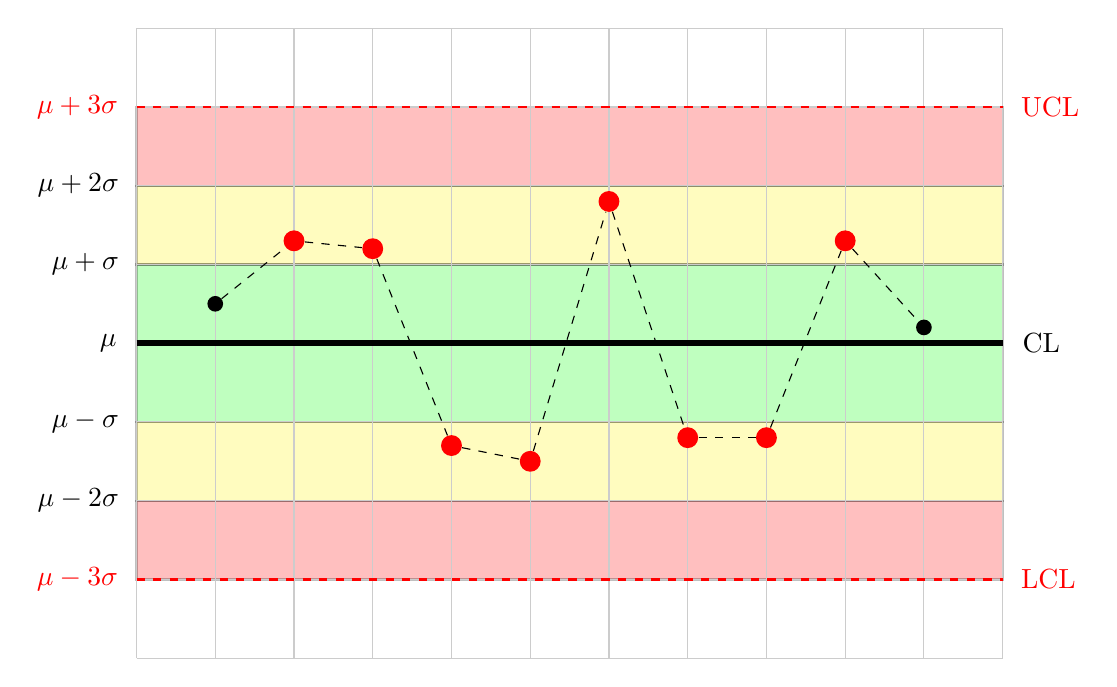
\begin{tikzpicture}[scale=1]
\draw[black, thick, fill=green,opacity=0.25] (0,-1) rectangle (11, 1);
\draw[black, thick, fill=yellow,opacity=0.25] (0,-2) rectangle (11, -1);
\draw[black, thick, fill=yellow,opacity=0.25] (0,1) rectangle (11, 2);
\draw[black, thick, fill=red,opacity=0.25] (0,-3) rectangle (11, -2);
\draw[black, thick, fill=red,opacity=0.25] (0,2) rectangle (11, 3);
\draw[thin,gray!40] (0,-4) grid (11,4);
\draw[line width=2pt](0,0)node[left=1mm]{$\mu$}--(11,0)node[right=1mm]{CL} ;
 \draw[line width=1pt,red, dashed](0,3)node[left=1mm]{$\mu+3\sigma$}--(11,3)node[right=1mm]{UCL};
\draw[line width=1pt,red, dashed](0,-3)node[left=1mm]{$\mu-3\sigma$}--(11,-3)node[right=1mm]{LCL};

\node[left=1mm] at (0,1){$\mu+\sigma$};
\node[left=1mm] at (0,-1){$\mu-\sigma$};
\node[left=1mm] at (0,2){$\mu+2\sigma$};
\node[left=1mm] at (0,-2){$\mu-2\sigma$};

 \node (A) at (1,0.5) [circle,fill=black,scale=0.6]{};
 \node (B) at (2,1.3) [circle,fill=red,scale=0.8]{};
 \node (C) at (3,1.2) [circle,fill=red,scale=0.8]{};
 \node (D) at (4,-1.3) [circle,fill=red,scale=0.8]{};
 \node (E) at (5,-1.5) [circle,fill=red,scale=0.8]{};
 \node (F) at (6,1.8) [circle,fill=red,scale=0.8]{};
\node (G) at (7,-1.2) [circle,fill=red,scale=0.8]{};
\node (H) at (8,-1.2) [circle,fill=red,scale=0.8]{};
\node (I) at (9,1.3) [circle,fill=red,scale=0.8]{};
\node (J) at (10,0.2) [circle,fill=black,scale=0.6]{};

\draw[-,dashed] (A)--(B); 
\draw[-,dashed] (B)--(C);
\draw[-,dashed] (C)--(D);
\draw[-,dashed] (D)--(E); 
\draw[-,dashed] (E)--(F);
\draw[-,dashed] (F)--(G); 
\draw[-,dashed] (G)--(H);
\draw[-,dashed] (H)--(I);
\draw[-,dashed] (I)--(J);

 \end{tikzpicture}
\end{center}

\begin{problem}\label{prob:controlChartWithSlider}
Suppose that a manufacturing process is known to have a normal distribution with a mean $\mu=3.5$, and standard deviation $\sigma=2$.  A random sample of size $n=4$ is collected every hour to monitor the manufacturing process.  The distribution of sample means (sampling distribution) will be normal and $$\mu_{\bar{x}}=\answer{3.5},\quad \sigma_{\bar{x}}=\answer{1}$$

Determine upper and lower control limits ($\pm 3\sigma$), for the $\bar{X}$-control chart for this manufacturing process.

$$LCL=\answer{0.5},\quad UCL=\answer{6.5}$$

The GeoGebra interactive below shows the means of consecutive samples $1$ through $32$ taken over the course of two days.  Use the scroll bar to navigate all samples and answer the questions below.

\begin{onlineOnly}
\begin{center}
\geogebra{jeu5trsd}{950}{650}
\end{center}
\end{onlineOnly}

What can you say about Samples  1-6:
\begin{multipleChoice}
    \choice{Everything looks good, keep the process going.}
    \choice{A point is above or below one of the control limits.}
    \choice[correct]{Two out of three consecutive points are in Zone 3.}
    \choice{Four out of five consecutive points are in Zone 2.}
    \choice{Eight consecutive points are on the same side of the center line.}
    \choice{Rising or falling pattern is exhibited by seven consecutive points.}
\end{multipleChoice}

What can you say about Samples  7-12:
\begin{multipleChoice}
    \choice{Everything looks good, keep the process going.}
    \choice[correct]{A point is above or below one of the control limits.}
    \choice{Two out of three consecutive points are in Zone 3.}
    \choice{Four out of five consecutive points are in Zone 2.}
    \choice{Eight consecutive points are on the same side of the center line.}
    \choice{Rising or falling pattern is exhibited by seven consecutive points.}
\end{multipleChoice}

What can you say about Samples  13-17:
\begin{multipleChoice}
    \choice{Everything looks good, keep the process going.}
    \choice{A point is above or below one of the control limits.}
    \choice{Two out of three consecutive points are in Zone 3.}
    \choice[correct]{Four out of five consecutive points are in Zone 2.}
    \choice{Eight consecutive points are on the same side of the center line.}
    \choice{Rising or falling pattern is exhibited by seven consecutive points.}
\end{multipleChoice}

What can you say about Samples  18-25:
\begin{multipleChoice}
    \choice{Everything looks good, keep the process going.}
    \choice{A point is above or below one of the control limits.}
    \choice{Two out of three consecutive points are in Zone 3.}
    \choice{Four out of five consecutive points are in Zone 2.}
    \choice[correct]{Eight consecutive points are on the same side of the center line.}
    \choice{Rising or falling pattern is exhibited by seven consecutive points.}
\end{multipleChoice}

What can you say about Samples  26-32:
\begin{multipleChoice}
    \choice{Everything looks good, keep the process going.}
    \choice{A point is above or below one of the control limits.}
    \choice{Two out of three consecutive points are in Zone 3.}
    \choice{Four out of five consecutive points are in Zone 2.}
    \choice{Eight consecutive points are on the same side of the center line.}
    \choice[correct]{Rising or falling pattern is exhibited by seven consecutive points.}
\end{multipleChoice}
\end{problem}

\subsection*{CASE STUDY: Thermoform production}

In thermoform production, sheets of plastic are heated and molded into a desired shape.  In the Desmos sheet below, we can see the diameters of 80 different thermoform spheres produced in Taiwan.  Notice that the last 20 were too big - something about the production had gone wrong.  Were there warning signs that a problem was coming before it happened?

\desmos{lwyjp4jqzh}{800}{600}

The following YouTube video gives some ideas of how we can use the Desmos sheet.

\youtube{NIg050X6q10}

Also included in the Desmos sheet are x-bar control charts for samples of size $n=3$ and $n=5$.  


\section*{Practice Problems}

\section*{References}
CASE STUDY on Thermoform Production is modified from:

MIT Open CourseWare \href{https://creativecommons.org/licenses/by-nc-sa/4.0/}{CC-BY-NC-SA}

Control of Manufacturing Processes (SMA 6303)

\href{https://ocw.mit.edu/courses/2-830j-control-of-manufacturing-processes-sma-6303-spring-2008/resources/ps3/}{Assignment 3}, \href{https://ocw.mit.edu/courses/2-830j-control-of-manufacturing-processes-sma-6303-spring-2008/resources/35/}{Part 5}. 

\end{document} 